\chapter{Prace nad architekturą i infrastrukturą projektu}
\label{cha:infra}


Niniejszy rozdział zawiera opis prac wykonanych przez autorów w ramach rozwoju architektury i infrastruktury systemu GGSS. Rozdział ten stanowi bezpośrednią kontynuację pracy inżynierskiej autorów, gdzie przygotowane zostały pierwsze wersje rozwijanych w ramach pracy magisterskiej rozwiązań. Przedstawione tu informację dotyczą szerokiego zakresu zagadnień związanych z inżynierią oprogramowania, takich jak: zarządzanie strukturą projektu oraz jego zależnościami, automatyzacja procesów towarzyszących wytwarzaniu oprogramowania czy przygotowanie infrastruktury ułatwiającej testy warstwy sprzętowej systemu. 

\section{Zmiany w architekturze projektu}
Przez zmiany w architekturze projektu autorzy rozumieją stopniowy rozwój zaimplementowanego przez nich w ramach pracy inżynierskiej rozwiązania. Rozwój ten obejmuje przede wszyskim uproszczenie powstałej hierarchii zależności między poszczególnymi elementami warstwy oprogramowania (rozumianymi zarówno jako repozytoria, jak i biblioteki), uczynienie systemu bardziej przystępnym dla użytkownika (np. poprzez nadanie komponentom nazw dobrze oddających ich przeznaczenie) oraz przygotowanie systemu pozwalającego w prosty sposób odtworzyć kod źródłowy w wersji bez wprowadzonych w ramach pracy magisterskiej modyfikacji (jako rodzaj zabezpieczenia przed skutkami potencjalnych błędów, które mogły zostać wprowadzone do oprogramowania podczas prac nad nim). Znaczna część zmian opisanych w niniejszej części pracy była możliwa do wprowadzenia z uwagi na trwające jednocześnie prace nad kodem źródłowym systemu GGSS i zmiany zachodzące w ich czasie.

\subsection{Wprowadzenie do problematyki}
Przeprowadzone przez autorów w ramach pracy inżynierskiej modyfikacje architektury systemu GGSS obejmowały przede wszystkim migrację projektu do systemu kontroli wersji Git, wprowadzenie spójnego nazewnictwa poszczególnych komponentów oraz zastosowanie funkcjonalności submodułów będącej częścią technologii Git do stworzenia hierarchicznej struktury repozytoriów (w odróżnieniu od pierwotnej, płaskiej architektury opartej o katalogi). Celem tych zmian było ułatwienie pracy nad pojedynczymi komponentami projektu oraz uczynienie struktury projektu przyjazną dla użytkownika, co zostało zdaniem autorów osiągnięte. 

Architektura stanowiąca punkt wyjściowy zmian wykonanych w ramach niniejszej pracy przedstawiona została na rysunku \ref{fig:old_structure} (z pominięciem repozytoriów pomocniczych, zawierających np. dokumentację). Projekt zawierał 14 repozytoriów, tworzących strukturę hierarchiczną, w skład których wchodziły m.in.: aplikacje, pomocnicze skrypty, infrastruktura budowania oraz kod źródłowy bibliotek implementujących poszczególne funkcjonalności systemu. W kontekście tej części pracy szczególnie istotne są repozytoria zawierające kod źródłowy bibliotek statycznych oraz pliki nagłówkowe, stanowiące trzon projektu (tzn. wykorzystywane przez aplikację \emph{ggss-runner}): \emph{ggss-lib}, \emph{ggss-software-libs}, \emph{ggss-hardware-libs}, \emph{ggss-util-libs} oraz \emph{ggss-misc} (repozytoria te oznaczone zostały na rys. \ref{fig:old_structure} kolorem niebieskim). Ich rola w pierwotnej wersji projektu prezentowała się następująco:
\begin{itemize}
    \item \textbf{\emph{ggss-hardware-libs}} - przechowywanie bibliotek odpowiedzialnych za obsługę urządzeń wchodzących w skład warstwy sprzętowej systemu GGSS. W pierwotnej wersji projektu były to następujące biblioteki statyczne:
    \begin{itemize}
        \item \emph{caenhv-lib} oraz \emph{caenn1470-lib} - odpowiedzialne za komunikację z zasilaczami wysokiego napięcia CAEN N1470
        \item \emph{mca-lib} oraz \emph{ortecmcb-lib} - odpowiedzialne za obsługę wielokanałowego analizatora amplitudy CAEN N957
        \item \emph{usbrm-lib} - odpowiedzialna za obsługę multipleksera sygnałów analogowych
    \end{itemize}
    \item \textbf{\emph{ggss-software-libs}} - przechowywanie bibliotek odpowiedzialnych za implementację wykorzystywanych przez system algorytmów i struktur danych związanych ściśle z warstwą oprogramowania (tzn. nie mających związku z warstwą sprzętową). W pierwotnej wersji projektu były to następujące biblioteki statyczne:
    \begin{itemize}
        \item \emph{xml-lib} - odpowiedzialna za implementację operacji odczytu oraz zapisu plików w formacie XML oraz operacji na strukturze drzewiastej powstałej w wyniku sparsowania zapisanych w tym formacie danych.
        \item \emph{fifo-lib} - odpowiedzialna za implementację prostej struktury danych, stanowiącej kolejkę typu FIFO (\emph{First In, First Out}) o ograniczonym rozmiarze.
        \item \emph{fit-lib} - odpowiedzialna za implementację operacji wykonywanych na zebranych przez system danych, w tym przede wszystkim za mechanizm dopasowania do nich krzywej.
        \item \emph{daemon-lib} - odpowiedzialna za implementację mechanizmu pozwalającego uruchomić aplikację \emph{ggss-runner} jako tzw. demon (ang. \emph{daemon}) - usługa działająca ,,w tle''
    \end{itemize}
    \item \textbf{\emph{ggss-util-libs}} - przechowywanie bibliotek, od których zależne są zarówno komponenty odpowiedzialne za obsługę warstwy sprzętowej projektu, jak i związane wyłącznie z warstwą oprogramowania. Innymi słowy, były to biblioteki wykorzystywane przez zawartość obu wyżej wymienionych repozytoriów, a zatem nie mogące znaleźć się w żadnym z nich. W pierwotnej wersji projektu były to następujące biblioteki statyczne:
    \begin{itemize}
        \item \emph{log-lib} - odpowiedzialna za implementację mechanizmu dziennika zdarzeń, zapisującego w plikach \lstinline{.log} informacje o zdarzeniach mających miejsce w systemie
        \item \emph{utils-lib} - odpowiedzialna za implementację pomniejszych funkcjonalności, takich jak konwersja między łańuchem znakowym a liczbą (przed pojawieniem się standardu C++11 tego typu funkcjonalności nie były częścią biblioteki standardowej)
        \item \emph{handle-lib} - odpowiedzialna za implementację wykorzystywanego w projekcie mechanizmu slotów i sygnałów
        \item \emph{thread-lib} - odpowiedzialna za implementację wykorzystywanego w projekcie mechanizmu wielowątkowości
    \end{itemize}
    \item \textbf{\emph{ggss-misc}} - przechowywanie plików nagłówkowych (niebędących cześcią żadnej z bibliotek statycznych) oraz plików \lstinline{.cmake} tworzących infrastrukturę budowania projektu
    \item \textbf{\emph{ggss-lib}} - przechowywanie kodu źródłowego zawierającego główną logikę systemu GGSS
\end{itemize}

\begin{landscape}

\begin{figure}
\centering
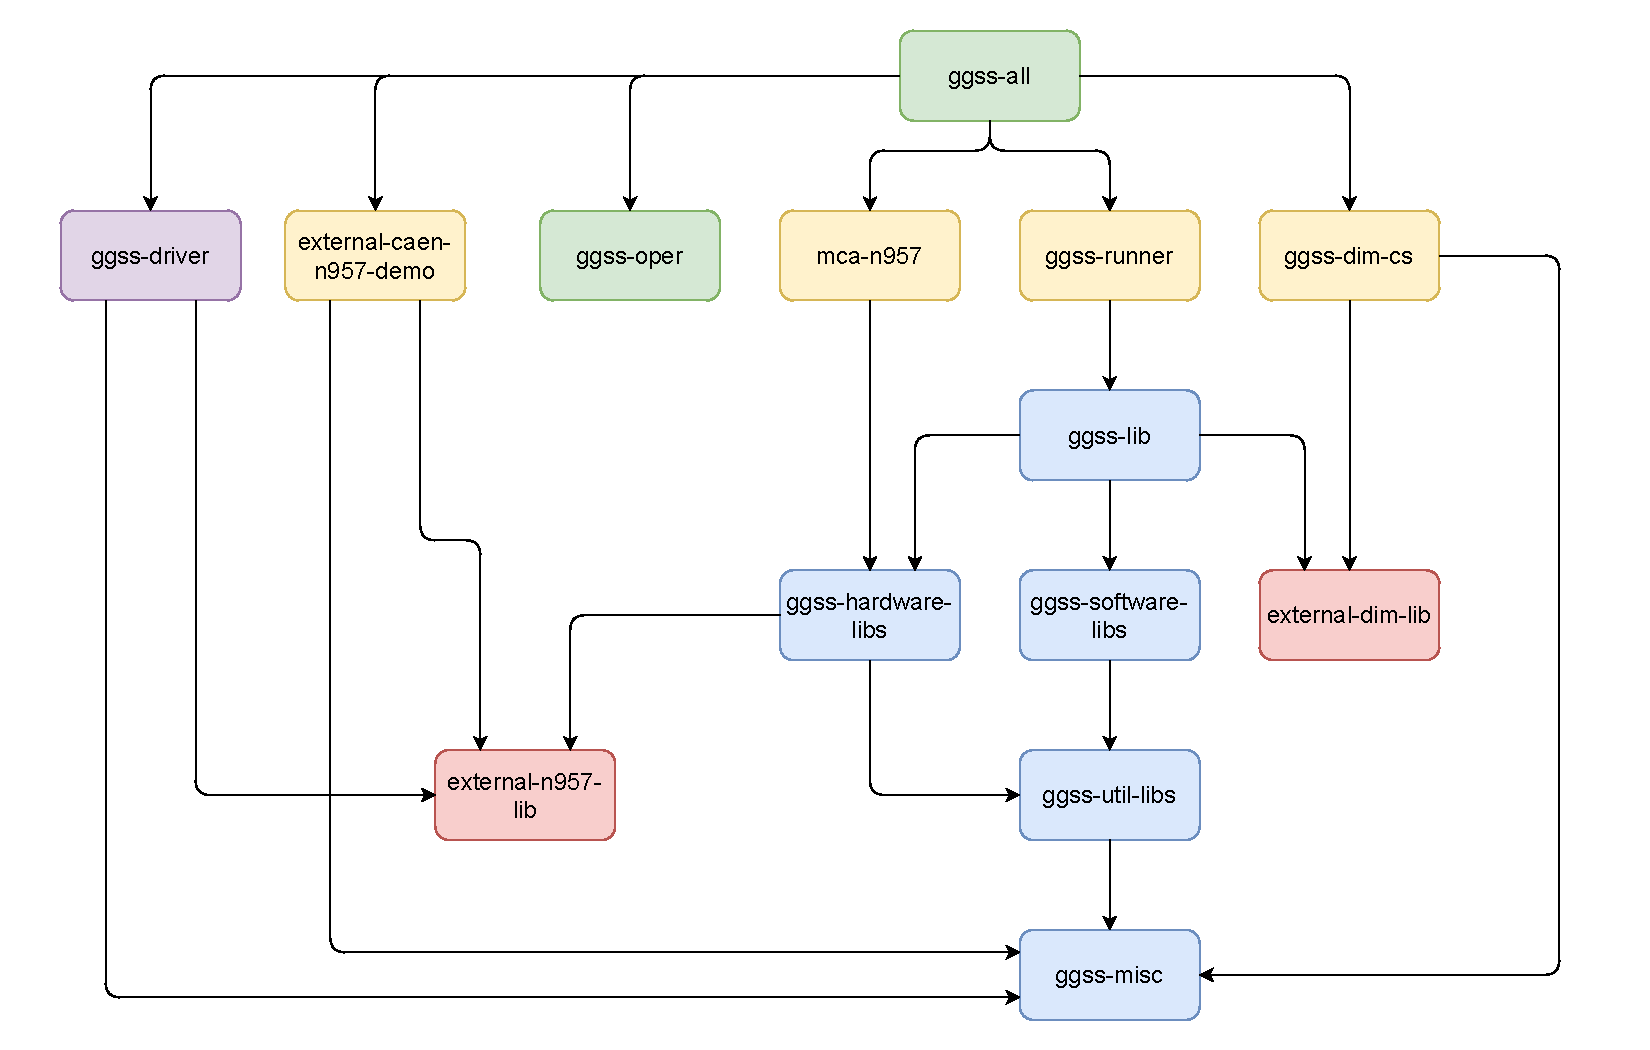
\includegraphics[width=1.35\textwidth]{components/infra_images/old_structure.pdf}
\caption{Architektura projektu przed wprowadzeniem modyfikacji (sytuacja wyjściowa). Groty strzałek wskazują repozytoria bazowe, kolory natomiast opisują rolę poszczególnych modułów: zielony oznacza repozytoria pomocnicze, żółty - aplikacje, czerwony - biblioteki zewnętrzne, fioletowy - sterownik a niebieski - biblioteki i pliki nagłówkowe projektu GGSS.}
\label{fig:old_structure}
\end{figure}

\end{landscape}

\subsection{Motywacja do wprowadzenia zmian}
Przygotowane przez autorów w ramach pracy inżynierskiej rozwiązanie było w pełni funkcjonalne, charakteryzowało się jednak pewnymi wadami i ograniczeniami, wynikającymi przede wszystkim z ograniczeń czasowych, niewielkiego doświadczenia autorów w pracy z projektem oraz istniejącego wtedy założenia o niemodyfikowaniu kodu źródłowego aplikacji i bibliotek wchodzących w skład projektu. Najważniejsze z występujących w tym rozwiązaniu problemów to:
\begin{itemize}
    \item głęboka hierarchia zależności, mająca negatywny wpływ na wydajność działania mechanizmu submodułów
    \item istnienie repozytorium \emph{ggss-misc}, zawierającego (poza szablonami CMake) elementy kodu źródłowego niepasujące do pozostałych bibliotek wchodzących w skład systemu: bazowe klasy wyjątków stosowanych w całym projekcie oraz flagi konfigurujące projekt w zależności od systemu operacyjnego (konieczność zastosowania tego typu zabiegu wynikła wprost z założenia o niemodyfikowaniu kodu źródłowego w czasie tworzenia pracy inżynierskiej)
    \item zachowanie oryginalnych nazw bibliotek i aplikacji, dostosowując je jedynie do przyjętej konwencji. Jedną z bibliotek wchodzących w skład projektu była biblioteka statyczna \emph{handle-lib}, odpowiedzialna za implementację mechanizmu slotów i sygnałów, na co, zdaniem autorów, jej nazwa nie wskazuje.
    \item wnioskowanie o zależnościach pomiędzy bibliotekami na podstawie dyrektyw preprocesora \emph{include} zawartych w kodzie źródłowym, a nie wykorzystywanych funkcjonalności, co wynikało z niewielkiego doświadczenia i wiedzy autorów na temat systemu podczas tworzenia pracy inżynierskiej oraz wspomnianego już założenia o niemodyfikowaniu kodu źródłowego.
    \item założenie o tworzeniu oddzielnego repozytorium dla każdej z występujących w projekcie aplikacji, niezależnie od jej rozmiarów, co ostatecznie znacznie skomplikowało powiązania pomiędzy repozytoriami (np. repozytoria \emph{external-caen-n957-demo} oraz \emph{mca-n957} charakteryzują się podobnymi zależnościami i oba zawierają niewielkie aplikacje, których zadaniem jest współpraca z wielokanałowym analizatorem amplitudy CAEN N957 - mogłoby być więc połączone w jedno repozytorium).
    \item brak łatwego sposobu na odtworzenie pierwotnej postaci kodu źródłowego - mechanizm ten nie był potrzebny na etapie pracy inżynierskiej, ponieważ nie dokonywano wtedy modyfikacji we wspomnianym kodzie.
\end{itemize}


\subsection{Uproszczenie architektury projektu}
Pierwszym podjętym przez autorów działaniem mającym na celu modyfikację struktury projektu była próba jej uproszczenia poprzez analizę zależności wewnętrzych systemu (tzn. zależności pomiędzy poszczególnymi bibliotekami). Prowadzone równolegle prace nad kodem źródłowym projektu pozwoliły autorom zaobserwować, iż pewna część występujących w nim dyrektyw preprocesora \lstinline{#include} nie oddaje w poprawny sposób faktycznej struktury zależności między bibliotekami. Najważniejszy przykład stanowi łańcuch zależności występujących pomiędzy biblioteką \emph{ggss-lib}, a bibliotekami \emph{caenhv-lib} oraz \emph{thread-lib}. W oryginalnej wersji projektu zależności między wymienionymi komponentami prezentowały się tak, jak na rysunku \ref{fig:dependency_problem_old}, tzn. bibliteka \emph{ggss-lib} zależna była od biblioteki \emph{caenhv-lib}, która natomiast zawierała dyrektywę \lstinline{#include} dołączającą plik nagłówkowy z biblioteki \emph{thread-lib}.


\savebox{\mybox}{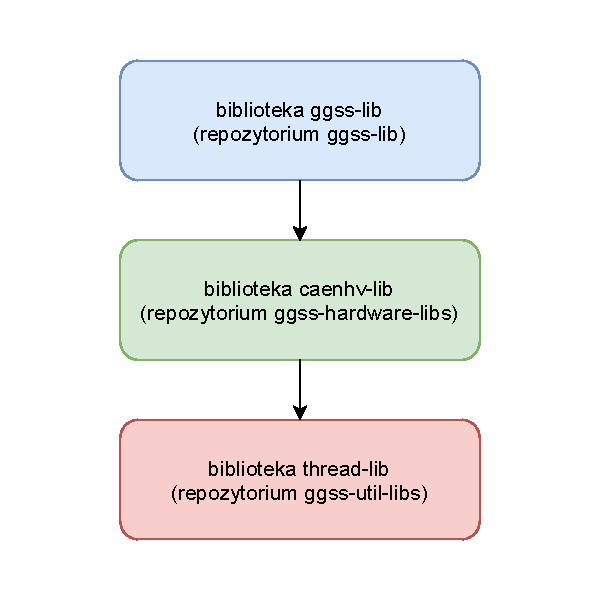
\includegraphics[width=0.40\textwidth]{components/infra_images/dependency_problem_old.pdf}}

\begin{figure}[H]
\centering
\begin{subfigure}[t]{0.40\textwidth}
\centering
\usebox{\mybox}
\caption{Oryginalna struktura.}
\label{fig:dependency_problem_old}
\end{subfigure}
\hfill
\begin{subfigure}[t]{0.55\textwidth}
\centering
\vbox to \ht\mybox{%
    \vfill
    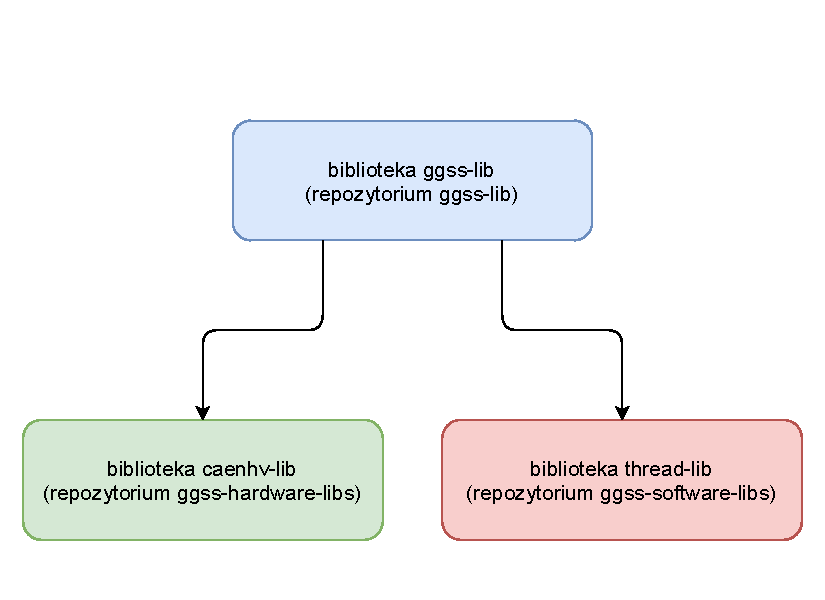
\includegraphics[width=\textwidth]{components/infra_images/dependency_problem_solution.pdf}
    \vfill
}
\caption{Struktura po wprowadzeniu zmian.}
\label{fig:dependency_problem_solved}
\end{subfigure}

\caption{Zestawienie oryginalnej oraz nowej struktury zależności pomiędzy bibliotekami \emph{ggss-lib}, \emph{caenhv-lib} oraz \emph{thread-lib}. Groty strzałek wskazują w stronę modułów bazowych.}
\end{figure}

W rzeczywistości biblioteka \emph{caenhv-lib} nie wykorzystywała zawartości wspomnianego pliku nagłówkowego - pełniła jedynie formę swego rodzaju pośrednika, udostępniając znajdujące się tam klasy bibliotece \emph{ggss-lib}. Przeniesienie dyrektywy \lstinline{#include} do biblioteki \emph{ggss-lib} spowodowało, iż żadna z bibliotek wchodzących w skład repozytorium \emph{ggss-hardware-libs} nie zawierała zależności do biblioteki \emph{thread-lib}. Rozwiązanie to pozwoliło dokonać migracji tejże biblioteki, wraz z wykorzystywaną przez nią biblioteką \emph{handle-lib}, do repozytorium \emph{ggss-software-libs}, redukując tym samym liczbę bibliotek znajdujących się w repozytorium \emph{ggss-util-libs}. Rysunek \ref{fig:dependency_problem_solved} przedstawia w sposób schematyczny strukturę otrzymanego rozwiązania.

W związku z opisanymi powyżej zmianami ilość kodu źródłowego znajdującego się w repozytorium \emph{ggss-util-libs} znacznie spadła - pozostałe tam biblioteki \emph{log-lib} oraz \emph{utils-lib} charakteryzowały się niewielkim rozmiarem. Spowodowało to, iż jednoczesne istnienie modułów \emph{ggss-misc} oraz \emph{ggss-util-libs} (po wprowadzonych zmianach spełniających tą samą rolę przechowywania niewielkiej liczby komponentów wykorzystywanych przez wiele modułów projektu GGSS) przestało być uzasadnione. Kolejny etap wykonanych prac stanowiło więc przeprowadzenie integracji tychże repozytoriów - w tym celu zdecydowano się na likwidację modułu \emph{ggss-misc} po wcześniejszym przeniesieniu jego zawartości do \emph{ggss-util-libs}.

Migracja znajdujących się w repozytorium \emph{ggss-misc} plików \lstinline{.cmake} (modułów wykorzystywanych przez infrastrukturę budowania projektu) wymagała, poza wykonaniem trywialnej czynności przeniesienia katalogu, aktualizacji (na poziomie całego projektu) ścieżek wskazujących lokalizację tychże plików. Działanie to było konieczne, ponieważ narzędzie CMake wymaga od programisty, by wyspecyfikował on lokalizację modułów \lstinline{.cmake} dołączanych do projektu (np. za pomocą komendy \lstinline{include()}) poprzez dodanie ścieżki z ich lokalizacją do listy \lstinline{CMAKE_MODULE_PATH} (przykład wykorzystania tejże listy przedstawiony został na listingu \ref{lst:module_path}). Oznaczało to więc konieczność wykonania, w każdym module wykorzystującym pliki \lstinline{.cmake}, zmiany wspomnianej ścieżki tak, by wskazywała na katalog \emph{cmake-templates} w repozytorium \emph{ggss-util-libs}.

\begin{lstlisting}[
    language=cmake,
    caption={Przykładowy fragment pliku \lstinline{CMakeLists.txt}, obrazujący sposób użycia listy \lstinline{CMAKE_MODULE_PATH} w celu wskazania lokalizacji plików zawierających często wykorzystywane w projekcie, pomocnicze funkcje.},
    label={lst:module_path}
]
# Przypisanie pojedynczej wartości (zawierającej ścieżkę do katalogu
# cmake-templates, w którym znajdują się wykorzystywane w projekcie
# pliki .cmake) do listy CMAKE_MODULE_PATH
set(CMAKE_MODULE_PATH "${CMAKE_CURRENT_LIST_DIR}/../ggss-util-libs/cmake-templates")

# Dołączenie znajdujących się w katalogu cmake-templates plików .cmake
include(BuildStaticLibrary)     # ggss_build_static_library
include(SetupTests)             # ggss_setup_tests

# Wykorzystanie znajdującej się w pliku .cmake funkcji
ggss_build_static_library(
    TARGET_NAME "fifo"
)
\end{lstlisting}


Poza wspomnianymi plikami \lstinline{.cmake} w repozytorium \emph{ggss-misc} znajdował się katalog \lstinline{include}, zawierający trzy pliki nagłówkowe z kodem napisanym w języku C++:
\begin{itemize}
    \item pliki \lstinline{ggssExceptions.h} oraz \lstinline{HardwareException.h} zawierające klasy bazowe wyjątków wykorzystywanych w całym projekcie GGSS
    \item plik \lstinline{CompatibilityFlags.h}, zawierający flagi konfigurujące projekt w zależności od platformy docelowej (Windows lub Linux)
\end{itemize}
Pliki te nie wchodziły oryginalnie w skład żadnej z bibliotek projektu GGSS, nie mogły zostać do nich również dodane przez autorów podczas przygotowywania pracy inżynierskiej, ponieważ wymagałoby to modyfikacji kodu źródłowego systemu. Podczas przeprowadzanej w ramach niniejszej pracy migracji tych plików do repozytorium \emph{ggss-util-libs} zdecydowano się na likwidację katalogu \lstinline{include} i rozdysponowanie jego zawartości do istniejących lub nowych bibliotek. Plik \lstinline{CompatibilityFlags.h} przeniesiony został więc do biblioteki \emph{utils-lib}, natomiast na potrzebę dwóch pozostałych nagłówków przygotowana została nowa biblioteka \emph{exceptions-lib}.

Finalna struktura repozytorium \emph{ggss-util-libs} przedstawiona została na listingu \ref{lst:util_final}. Poza wspomnianymi do tej pory zmianami nowość stanowi katalog \lstinline{doxygen-config}, zawierający prosty plik konfigurujący działanie narzędzia Doxygen służącego do generowania dokumentacji programów napisanych w języku C++. Rozszerzenie projektu o możliwość generowania dokumentacji zostanie jednak opisane szczegółowo w dalszej części pracy.

\begin{lstlisting}[
    caption={Zawartość repozytorium \emph{ggss-util-libs} po wprowadzeniu opisanych zmian. Widoczne są biblioteki wchodzące w skład repozytorium: \emph{exceptions-lib}, \emph{log-lib} oraz \emph{utils-lib}, katalog \emph{cmake-templates} zawierający szablony wykorzystywane przez system budowania, katalog \emph{doxygen-config} zawierający konfigurację narzędzia Doxygen, nadrzędny plik \emph{CMakeLists.txt} służący do budowania wszystkich bibliotek w repozytorium oraz plik \emph{README.md} zawierający opis repozytorium.},
    label={lst:util_final}
]
.
|-- CMakeLists.txt
|-- README.md
|-- cmake-templates
|-- doxygen-config
|-- exceptions-lib
|-- log-lib
`-- utils-lib
\end{lstlisting}

Poza wspomnianymi do tej pory repozytoriami zmianami objęte zostały ponadto moduły przechowujące aplikacje służące do testowania i obsługi urządzeń elektronicznych wchodzących w skład warstwy sprzętowej systemu GGSS. Motywacją do wprowadzenia modyfikacji była konieczność rozbudowy projektu o kolejne tego typu aplikacje - tworzenie dla każdej z nich osobnego repozytorium znacząco komplikowałoby strukturę projektu. Zdecydowano zatem, iż repozytoria \emph{mca-n957} oraz \emph{external-caen-n957-demo} zostaną dołączone do nowo powstałego repozytorium \emph{ggss-hardware-service-apps}, grupującego niewielkie programy służące do operowania na urządzeniach.


% TODO: moze wspomniec o koniecznosci zachowania historii i jak zostało to zrobione???

Poza zmniejszeniem progu wejścia do projektu poprzez uczynienie jego struktury prostszą, opisane do tej pory zmiany korzystnie wpłynęły na działanie mechanizmu submodułów systemu Git, na którym oparty został proces zarządzania zależnościami między repozytoriami w projekcie. Redukcja liczby repozytoriów i powiązań między nimi oraz zmniejszenie głębokości drzewa zależności (poprzez likwidację repozytorium \emph{ggss-misc}) miało pozytywny wpływ na wydajność systemu zarządzającego architekturą projektu. 



\subsection{Dodanie możliwości odtworzenia pierwotnej wersji kodu źródłowego}
Wprowadzanie zmian w kodzie źródłowym aplikacji, której jedną z najważniejszych cech jest jej niezawodność, stanowi znaczące ryzyko. Tego typu aplikacją jest program \emph{ggss-runner}, stanowiący trzon projektu GGSS, a którego źródła podlegały modyfikacjom w ramach opisanych w niniejszym manuskrypcie prac. Naturalnym było więc stworzenie mechanizmu pozwalającego na stosunkowo łatwy powrót do oryginalnej wersji aplikacji, tzn. takiej niezawierającej opisanych w niniejszej pracy zmian w kodzie źródłowym.

Możliwość odtworzenia pierwotnej wersji kodu źródłowego osiągnięta została poprzez utworzenie, dla każdego repozytorium biorącego udział w procesie budowania aplikacji \emph{ggss-runner}, specjalnej gałęzi nazwanej \emph{legacy}. Gałęzie te zawierają oryginalną wersję kodu źródłowego napisanego w języku C++, natomiast pozostałe elementy (infrastruktura budowania oraz ciągłej integracji i dostarczania) znalazły się tam w swoich najnowszych wersjach, co gwarantuje ich spójność w całym projekcie (a co za tym idzie, mogą być używane w taki sam sposób, jak na gałęzi głównej).

Opisanymi zmianami objęte zostały następujące repozytoria: \emph{ggss-all}, \emph{ggss-runner}, \emph{ggss-lib}, \emph{ggss-software-libs}, \emph{ggss-hardware-libs}, \emph{external-dim-lib}, \emph{external-n957-lib} oraz \emph{ggss-util-libs}. W przypadku repozytorów o nazwach zawierających przedrostek \emph{external-} zmiany te polegały jedynie na utworzeniu nowej gałęzi - zawartość bibliotek zewnętrznych nie była przez autorów pracy modyfikowana.

Ostatecznie więc zbudowanie aplikacji \emph{ggss-runner} w jej pierwotnej wersji jest bardzo proste, z poziomu repozytorim \emph{ggss-all} sprowadza się do wykonania komend zamieszczonych na listingu \ref{lst:legacy}. Dodatkowo, pliki \emph{README.md} stanowiące dokumentację poszczególnych repozytorów zostały na gałęziach \emph{legacy} odpowiednio zmodyfikowane, by opisywać obowiązującą tam procedurę budowania projektu oraz zawartość poszczególnych modułów.

\begin{lstlisting}[
    caption={Komendy pozwalające na pobranie kodu źródłowego oraz zbudowanie aplikacji \emph{ggss-runner} w jej oryginalnej wersji. },
    label={lst:legacy}
]
git clone ssh://git@gitlab.cern.ch:7999/atlas-trt-dcs-ggss/ggss-all.git &&
mkdir ggss-all-build &&
cd ggss-all &&
git checkout legacy &&
git submodule update --init --recursive &&
git submodule foreach --recursive git checkout legacy &&
cd ../ggss-all-build &&
python ../ggss-all/build.py --staticboost --buildtype release
\end{lstlisting}

\subsection{Pomniejsze zmiany}
Poza do tej pory opisanymi, wykonanych zostało kilka pomniejszych modyfikacji mających na celu szeroko pojętą poprawę jakości struktury projektu. Przeprowadzone prace obejmują bogaty zakres wprowadzonych zmian, nie jest więc możliwe zamieszczenie w niniejszej pracy dokładnego opisu każdej z nich. Poniżej krotko opisane zostały więc trzy wybrane przez autorów modyfikacje, charakteryzujące się różnym poziomem skomplikowania, ale operujące na poziomie pojedynczych repozytoriów. 

\subsubsection{Likwidacja repozytorium \emph{ggss-oper}}
Jednym z repozytoriów wprowadzonych przez autorów w ramach wykonywania pracy inżynierskiej był moduł \emph{ggss-oper}, zawierający skrypty oraz pliki konfiguracyjne stanowiące znaczną część infrastruktury przeznaczonej do użytkowania wraz z oprogramowaniem GGSS na maszynie docelowej. Zawartość tego repozytorium, nie stanowiąca wkładu wniesionego przez autorów niniejszej pracy w system, obejmowała m.in.: 
\begin{itemize}
    \item pierwsze wersje skryptów służących do przeprowadzania testów urządzeń wchodzących w skład warstwy sprzętowej projektu (napisane z wykorzystaniem języka Python)
    \item skrypty zarządzające stanem środowiska docelowego (np. ustawiające wymagane zmienne środowiskowe)
    \item skrypty zarządzające oprogramowaniem systemu GGSS, np. \lstinline{ggss_monitor.sh} pozwalający na uruchamianie, zatrzymywanie oraz sprawdzanie stanu aplikacji \emph{ggss-runner}
\end{itemize}
Wraz z postępami prac nad projektem, część z wymienionej powyżej zawartości zastąpiona została przez autorów pracy rozwiązaniami alternatywnymi (np. skrypty służące do przeprowadzania operacji na urządzeniach zastąpione zostały aplikacjami napisanymi w języku C++), pozostałe przeniesione zostały natomiast do repozytorium \emph{ggss-all}. Ostatecznie moduł został więc zlikwidowany.


\subsubsection{Utworzenie biblioteki \emph{asyncserial-lib}}
Podczas prac nad kodem źródłowym bibliotek statycznych wchodzących w skład repozytorium \emph{ggss-hardware-libs} zaobserwowano, że w katalogach bibliotek \emph{usbrm-lib} oraz \emph{caenn1470-lib} zamieszczony został, poza właściwym dla nich kodem źródłowym, zestaw plików zawierających implementację asynchronicznej komunikacji z urządzeniami za pomocą interfejsu szeregowego. Ponieważ znalezione w obu przypadkach pliki nie różniły się od siebie, i jednocześnie stanowiły niezbędny element wspomnianych komponentów systemu (zawierały kluczową dla działania projektu funkcjonalność), zdecydowano o utworzeniu nowej biblioteki zawierającej omawiane pliki. Biblioteka nazwana została, zgodnie ze swoim przeznaczeniem, \emph{asyncserial-lib} i weszła w skład repozytorium \emph{ggss-hardware-libs}.


\subsubsection{Zmiana nazwy biblioteki \emph{handle-lib}}
Jedną z bibliotek będących częścią systemu GGSS była biblioteka \emph{handle-lib}, odpowiedzialna za implementację mechanizmu slotów i sygnałów. Oryginalnie biblioteka ta znajdowała się w repozytorium \emph{ggss-util-libs}, jednak wraz z postępem prac przeniesiona została, wraz z biblioteką \emph{thread-lib}, do repozytorium \emph{ggss-software-libs}. Nazwa biblioteki nie pozwalała użytkowniki domyślić się, jakie jest jej zastosowanie - z tego powodu zdecydowano się wprowadzić nową nazwę: \emph{sigslot-lib} (od angielskiego \emph{signals and slots}).


\subsection{Podsumowanie}
W ramach przeprowadzonych prac wykonane zostały zmiany pozwalające na uproszczenie architektury projektu, czyniąc ją przyjaźniejszą dla użytkownika. Finalna struktura przedstawiona została na rysunku \ref{fig:new_architecture} (podobnie jak w przypadku hierarchii wyjściowej - z pominięciem repozytoriów pomocniczych, nie wchodzących bezpośrednio w jej skład) - aktualnie składa się ona z 11 repozytoriów.

\begin{figure}[H]
\centering
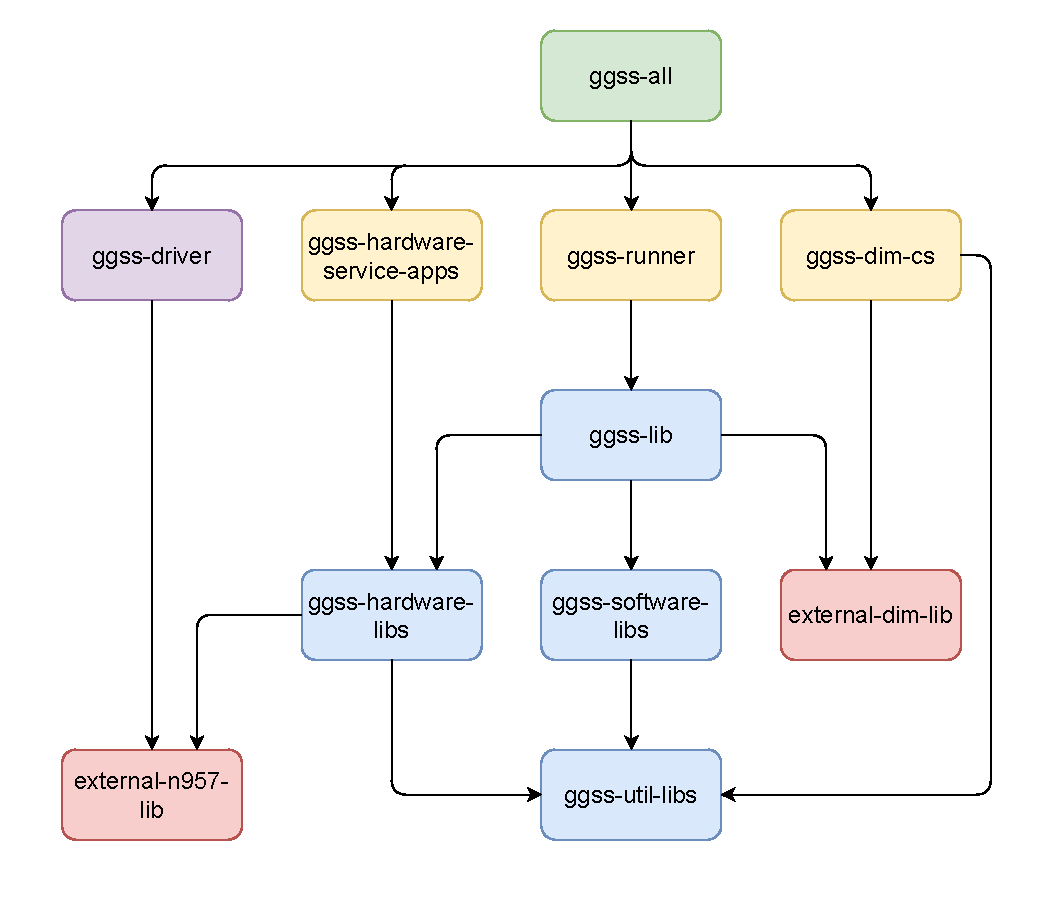
\includegraphics[width=\textwidth]{components/infra_images/new_architecture.pdf}
\caption{Finalna struktura projektu, po wprowadzeniu wszystkich zmian opisanych w niniejszej pracy. Strzałki wskazują w stronę modułów bazowych. Widoczne jest znaczące uproszczenie struktury projektu względem wersji oryginalnej (rys. \ref{fig:old_structure}).}
\label{fig:new_architecture}
\end{figure}

Dla repozytoriów biorących udział w procesie budowania aplikacji \emph{ggss-runner} utworzone zostały ponadto gałęzie \emph{legacy}, zawierające kod źródłowy projektu bez wprowadzonych w ramach niniejszej pracy zmian - dzięki temu możliwy jest stosunkowo łatwy powrót do oryginalnej wersji aplikacji, co stanowi zabezpieczenie na wypadek wprowadzenia do jej źródeł błędów.

\clearpage
\section{Automatyzacja pracy z submodułami (JC)}
\label{sec:gitio}

Ninejszy rozdział jest poświęcony obsługi wielopoziomowej struktury opartej o \emph{git submodules} obecnej w projekcie GGSS. Przedstawione zostaną plusy oraz minusy zastosowanego w trakcie pracy inżynierskiej rozwiązania. Omówiona zostanie przygotowana przez autorów infrastruktura mająca na celu ułatwienie pracy z submodułami. Dodatkowo krótko zostanie opisane przygotowane \emph{how-to} oraz praktyki które powinno się stosować pracując z taką architekturą.

\subsection{Wprowadzenie do problematyki}

W trakcie pracy inżynierskiej, a konkretnie migracji całego projektu GGSS do systemu kontroli wersji \emph{git} zdecydowano się na wykorzystanie technologii \emph{git submodules}. Ze względu na nacisk na zwiększenie modularyzacji projektu technologia ta idealnie wpasowywała się w docelową architekurę. Zasada działania submodułów jest bardzo zbliżona do dowiązań symbolicznych stosowanych między innymi w systemach UNIX. Zamiast wskazywać na ścieżkę do folderu na lokalnym systemie submoduł wskazuje na ścieżkę do konkretnej wersji repozytorium na zewnętrznym serwerze od którego zależy nasz moduł. Rysunek \ref{fig:submodules_links} przedstawia zasadę działania submodułów oraz wpływ wersjonowania na tenże mechanizm. Wykorzystanie submodułów pozwala na w pełni odseparowaną pracę nad wybranym komponentem systemu. Nie potrzebujemy pobierać żadnych dodatkowych plików, czy też zależności w celu zmienienia kodu źródłowego. Rozwiązanie to pozwala też na skorzystanie z bardzo szybkiej inicjalizacji całego projektu jedną komendą, co zostało przedstawione w listingu \ref{lst:initialize}.

\begin{figure}[H]
    \centering
    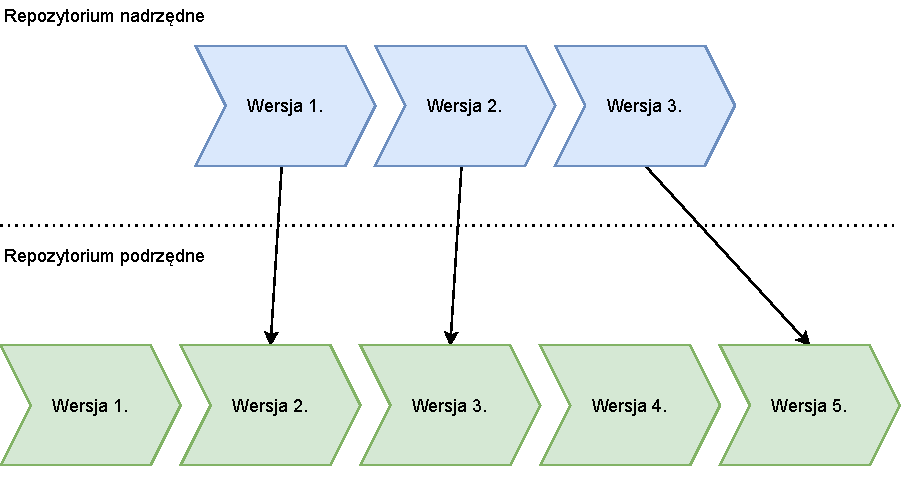
\includegraphics[width=0.9\textwidth]{submodule_links.pdf}
    \caption{Zasada działania submodułów.}
    \label{fig:submodules_links}
\end{figure}

\begin{lstlisting}[language=c++, caption={Inicjalizacja pełnej sturktury projektu jedną komendą.}, label={lst:initialize}]
root@host:/# git clone ssh://git@gitlab.cern.ch:7999/atlas-trt-dcs-ggss/ggss-all.git && cd ggss-all && git submodule update --init --recursive
Cloning into '/CERN/ggss-all/ggss-dim-cs'...
Cloning into '/CERN/ggss-all/ggss-driver'...
Cloning into '/CERN/ggss-all/ggss-oper'...
Cloning into '/CERN/ggss-all/ggss-runner'...
Cloning into '/CERN/ggss-all/ggss-spector'...
Cloning into '/CERN/ggss-all/mca-n957'...
Cloning into '/CERN/ggss-all/ggss-dim-cs/external-dim-lib'...
Cloning into '/CERN/ggss-all/ggss-dim-cs/ggss-misc'...
Cloning into '/CERN/ggss-all/ggss-driver/external-n957-lib'...
Cloning into '/CERN/ggss-all/ggss-driver/ggss-misc'...
...(13 lines truncated)
\end{lstlisting}


\subsection{Motywacja do wprowadzenia zmian}

Pomimo wielu aspektów \emph{git submodules}, które bardzo dobrze wpasowały się w, kreowaną przez autorów w trakcie pracy inżynierskiej, sturkturę technologia ta posiada też swoje minusy. Pierwszy znaczącym problemem napotkanym w trakcie pracy z submodułami było nietypowe zachowanie repozytoriów w trakcie ich inicjalizacji, a konkretnie automatyczne odłączanie ich od głównej gałęzi. Co więcej praca z submodułami wymaga od programisty zwiększonej czujności oraz stosowania dodatkowych zasad, ponieważ więcej jest miejsc na pomyłkę, co może doprowadzić do niepoprawnego działania wykorzystanych narzędzi. Kolejnym problemem napotkanym w trakcie pracy z submodułami jest czasochłonność niektórych operacji, w szczególności aktualizacji repozytorium na samym dole ``drzewa zależności``. Zmiana taka wymaga ręcznej aktualizacji po kolei każdego z repozytorium, aż do samej góry tejże skruktury co przedstawia rysunek \ref {fig:submodules_update}. Każda z aktualizacji przedstawiona na wyżej wymieionym rysunku, to tak na prawdę cztery lub więcej akcji do których wliczają się: aktualizacja repozytorium podrzędnego, dodanie wszystkich zmian do rejestru odpowiedzialnego za ich śledzenie, utworzenie nowej wersji repozytorium, opublikowanie nowej wersji na zewnętrznym serwerze.



\clearpage
\begin{figure}[H]
    \centering
    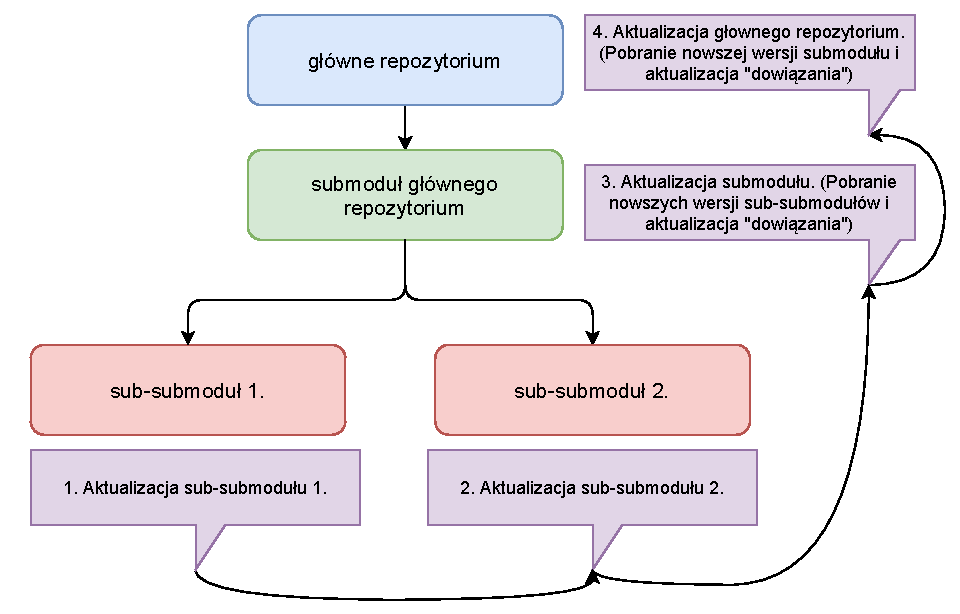
\includegraphics[width=0.9\textwidth]{submodules_update.pdf}
    \caption{Przykładowa architektura oparta o submoduły z krokami jakie należy podjąć, aby wprowadzić zmiany na ``najniższym`` poziomie.}
    \label{fig:submodules_update}
\end{figure}


\subsection{Automatyzacja z użyciem GITIO}

Problemem, którego rozwiązanie pochłonęło najwięcej czasu i wymagało największego wkładu pracy przez autorów było monotonne, wielokrokowie wprowadzanie zmian do projektu, szczególnie u dołu struktury zależności. W celu rozwiązanie tego problemu przygotowano aplikacje \emph{gitio} z wykorzystaniem języka \emph{Python}. Ze względu na to, że metadane technologii \emph{git} są bardzo złożone, a opanowanie zasad węwnętrznego działania tejże technologii wymagałoby bardzo dużo czasu skorzystano z dedykowanej, do tej technologii, bilbioteki napisanej również w języku \emph{Python}.

Zasada działania aplikacji jest dosyć prosta, natomiast znacząco ułatwia działania z wielopoziomową strukturą opartą o \emph{git submodules}. Argumenty wejściowe jako przyjmuje \emph{gitio} to:
\begin{itemize}
    \item \lstinline{-h, --help} - pozwala na wyświetlnie informacji o przeznaczeniu programu oraz przyjmowanych argumentach wraz z krótkim opisem
    \item \lstinline{-p PATH, --path PATH} -
    \item \lstinline{-b BIN, --bin BIN} -
\end{itemize}

\subsection{Dokumentacja sposobu pracy z submodułami}



\clearpage
\section{Rozwój systemu budowania projektu}
\label{ch:building_project}

Pierwsze w~pełni przystosowane do pracy z~opartą o~mechanizm submodułów strukturą projektu wydanie systemu budowania aplikacji oraz bibliotek wchodzących w~skład warstwy oprogramowania GGSS przygotowane zostało przez autorów w~ramach napisanej przez nich pracy inżynierskiej. Spełniało ono wszystkie podstawione przed nim wtedy wymagania, takie jak możliwość niezależnego budowania pojedynczych komponentów projektu. Jednakże wraz z~kontynuacją przez autorów prac nad projektem w~ramach niniejszej pracy magisterskiej, pojawiła się możliwość rozwoju stworzonego systemu, co pozwoliłoby uczynić go bardziej niezawodnym i~przyjaźniejszym dla użytkownika. Na kolejnych stronach manuskryptu opisane zostały zatem zmiany w~systemie budowania projektu GGSS, wprowadzone przez autorów w~czasie przygotowywania niniejszej pracy dyplomowej.

\subsection{Wprowadzenie do problematyki}
Przygotowany w~ramach pracy inżynierskiej system budowania oparty został o~narzędzie CMake oraz, w~mniejszym stopniu, o~proste skrypty napisane w~języku Python. Rezultatem było w~pełni działające rozwiązanie, spełniające wszystkie postawione wtedy przed nim wymagania:
\begin{itemize}
    \item niezależność od platformy - system powinien działać poprawnie zarówno na urządzeniach wykorzystujących system operacyjny Linux, jak i~na komputerach z~Windowsem.
    \item możliwość budowania projektu o~skomplikowanej, hierarchicznej strukturze, jakiego jak aplikacja \emph{ggss-runner} wchodząca w~skład warstwy oprogramowania GGSS 
    \item możliwość budowania każdego z~komponentów systemu z~osobna, bez wykorzystywania pozostałych, niepowiązanych z~nim modułów
    \item czytelna, jednopoziomowa (brak zagnieżdżeń) wynikowa struktura katalogów, w~której każdy zbudowany komponent znajduje się tylko raz, niezależnie od tego, jak wiele modułów było od niego zależnych
\end{itemize}

Ponieważ oprogramowanie systemu GGSS składa się z~wielu bibliotek i~aplikacji, dla których proces tworzenia przebiega bardzo podobnie, zdecydowano się zastosować rozwiązanie pozwalające na ponowne wykorzystanie poszczególnych komponentów systemu budowania. W~tym celu wykorzystywane często funkcjonalności wyodrębnione zostały w~postaci osobnych plików \lstinline{.cmake}. W~ten sposób do osobnych plików wydzielony został kod odpowiedzialny m.in. za: budowanie bibliotek statycznych, budowanie zależności danego komponentu czy dołączanie do projektu bibliotek Boost i~GSL. Następnie tego typu pliki (zwane w~dalszej części pracy szablonami CMake) wykorzystywane były w~plikach \lstinline{CMakeLists.txt} odpowiedzialnych za budowanie poszczególnych komponentów projektu, co zostało zobrazowane w~formie przykładu na listingu \ref{lst:cmake_old}. Zaprezentowany fragment kodu zawiera konfigurację procesu budowania biblioteki \emph{thread-lib}, wraz z~komentarzami w~języku polskim. 

\lstinputlisting[
    language=CMake, 
    caption={Fragment wykorzystywanego w~pierwotnej wersji systemu budowania pliku \lstinline{CMakeLists.txt} zawierający konfigurację procesu tworzenia biblioteki \emph{thread-lib}. Widoczne są przyjęte podczas tworzenia pracy inżynierskiej konwencje dotyczące sposobu wykorzystywania szablonów CMake. }, 
    label={lst:cmake_old}
]{4_infrastructure/code_samples/sample_old_cmake.cmake}

Przykład obrazuje sposób wykorzystywania szablonów CMake, jaki przyjęty został przez autorów podczas tworzenia przez nich pracy inżynierskiej - załączenie pliku za pomocą komendy \lstinline{include()} powodowało zamieszczenie znajdujących się w~nim instrukcji bezpośrednio w~danym miejscu kodu. Dodatkowo, jeśli zawartość tego typu pliku wymagała od użytkownika wyspecyfikowania dodatkowych informacji, takich jak lista koniecznych do zbudowania zależności, następowało to po prostu poprzez utworzenie (przed miejscem załączenia pliku) zmiennej o~odpowiedniej nazwie - na załączonym przykładzie jest to widoczne w~przypadku pliku \lstinline{BuildDependencies.cmake}, wymagającego do poprawnego działania istnienia zmiennych \lstinline{dependency_prefix} oraz \lstinline{dependencies}.

\subsection{Motywacja do wprowadzenia zmian}
Przygotowane przez autorów w~ramach pracy inżynierskiej rozwiązanie charakteryzowało się pewnymi ograniczeniami, takimi jak brak wsparcia dla testów jednostkowych oraz tworzenia dokumentacji kodu źródłowego za pomocą narzędzia Doxygen. Niewątpliwą wadą przygotowanego rozwiązania był ponadto sposób wykorzystywania szablonów CMake, wymagający od użytkownika znajomości ich zawartości (by wiedzieć, jakie zmienne powinny zostać utworzone, by system działał poprawnie). Znacznie bardziej przyjazną dla użytkownika alternatywą wydaje się być wykorzystanie funkcji i~makr, gdzie wszystkie potrzebne informacje przekazywane byłyby w~formie argumentów. Ponadto wraz z~pojawianiem się w~warstwie oprogramowania systemu GGSS kolejnych aplikacji konieczne stało się rozbudowanie skryptu \lstinline{build.py}, znajdującego się w~repozytorium \emph{ggss-all} i~odpowiadającego za wysokopoziomowe zarządzanie procesem budowania (m.in. wybór między wersja \emph{debug} i~\emph{release} oraz statycznym i~dynamicznym linkowaniem bibliotek wchodzących w~skład pakietu Boost).

\subsection{Zastosowanie funkcji i makr narzędzia CMake}
Jedną z~wprowadzonych podczas prac nad systemem budowania projektu GGSS zmian była przebudowa istniejących plików \lstinline{.cmake} poprzez umieszczenie znajdującego się tam kodu w~starannie nazwanych funkcjach i~makrach. Celem tej modyfikacji było ułatwienie osobom rozwijającym system GGSS dodawania nowych bibliotek i~aplikacji. Jak zostało wyżej wspomniane, przed wprowadzeniem omawianej modyfikacji do sprawnego korzystania z~przygotowanych szablonów konieczna była znajomość ich zawartości, ponieważ oczekiwały one często wyspecyfikowania wymaganych informacji za pomocą odpowiednio nazwanych zmiennych. Zamiast tego zaproponowane zostało rozwiązanie, w~którym wszystkie potrzebne informacje przekazywane są do odpowiedzialnej za daną operację funkcji (lub makra) poprzez nazwane argumenty wywołania. Z~punktu widzenia narzędzia CMake funkcjonalność taka dostępna jest przy pomocy komendy \lstinline{cmake_parse_arguments}. Ze względu na trywialny i~powtarzalny charakter wprowadzonych w~szablonach CMake przekształceń, w~niniejszej pracy pominięty został opis implementacji nowego rozwiązania, wskazana została natomiast różnica widoczna z~perspektywy osoby wykorzystującej istniejący system budowania. Na listingu \ref{lst:cmake_new} przedstawiony został przykład wykorzystania jednej ze stworzonych przez autorów funkcji: \lstinline{ggss_build_static_library} pochodzącej z~szablonu \lstinline{BuildStaticLibrary.cmake}. Przedstawiony fragment kodu wykonuje dokładnie to samo zadanie, co widoczny wcześniej na listingu \ref{lst:cmake_old} - odpowiedzialny jest za konfigurację procesu budowania biblioteki \emph{thread-lib}. Jest on znacznie krótszy od widocznego w~poprzednim przykładzie - zostało to osiągnięte poprzez przeniesienie do wnętrza funkcji funkcjonalności takich jak sprawdzenie, czy dany komponent został już przetworzony. Widoczny w~przykładzie sposób przekazywania informacji za pomocą nazwanych argumentów funkcji (np. \lstinline{DEPENDENCIES}) jest zdaniem autorów znacznie czytelniejszy od mechanizmu istniejącego w~projekcie wcześniej. Ponadto, dzięki wykorzystaniu funkcji, przedstawiony fragment przypomina kod źródłowy napisany za pomocą popularnych języków programowania, takich jak C~i C++, co zdaniem autorów czyni go bardziej intuicyjnym.

\lstinputlisting[
    language=CMake, 
    caption={Fragment wykorzystywanego w~najnowszej wersji systemu budowania pliku \lstinline{CMakeLists.txt} odpowiedzialnego za konfigurację procesu tworzenia biblioteki \emph{thread-lib}. Widoczne jest wykorzystanie funkcji oraz nazwanych argumentów w~celu zwiększenie czytelności prezentowanego kodu.}, 
    label={lst:cmake_new}
]{4_infrastructure/code_samples/sample_new_cmake.cmake}

W~sposób podobny do załączanego w~przykładzie pliku \lstinline{BuildStaticLibrary.cmake} zmodyfikowane zostały pozostałe wchodzące w~skład projektu pliki \lstinline{.cmake} (np. plik \lstinline{BuildDependencies.cmake}, odpowiedzialny za konfigurację zależności danego modułu) dzięki czemu wzrosła jakość kodu wchodzącego w~skład systemu budowania. W~większości przypadków autorzy zdecydowali się na wykorzystanie funkcji - zastąpienie ich za pomocą makr konieczne było tylko w~kilku szczególnych przypadkach. Najważniejszą różnicą między obiema wspomnianymi konstrukcjami jest fakt, iż w~ciele funkcji, w~przeciwieństwie do marka, tworzony jest nowy zasięg widoczności zmiennych (ang. \emph{scope}), przez co skutki zachodzących w~jej wnętrzu zmian, takich jak przypisania, nie są domyślnie widoczne poza nią. Zastosowane zmiany zgodne są ponadto z~konwencją, wedle której napisany za pomocą narzędzia CMake kod systemu budowania powinien być traktowany na równi z~kodem źródłowym przetwarzanych przez niego aplikacji i~bibliotek. 

\subsection{Wsparcie dla testów jednostkowych i dokumentacji}
Kolejną wprowadzoną przez autorów modyfikacją było dodanie, na poziomie systemu budowania, wsparcia dla testów jednostkowych oraz generowania, za pomocą narzędzia Doxygen, dokumentacji kodu źródłowego. Ponieważ obie wprowadzone funkcjonalności wykorzystywane są przez wiele komponentów projektu, ich implementacja zamieszczona została w~znajdujących się aktualnie w~repozytorium \emph{ggss-util-libs} plikach \lstinline{.cmake}, kolejno: \lstinline{SetupTests.cmake} i~\lstinline{SetupDoxygen.cmake}. Zgodnie ze stosowaną w~projekcie konwencją, również te funkcjonalności zaimplementowane zostały w~postaci funkcji (w~przypadku dokumentacji) oraz makra (w~przypadku testów, gdzie zostało to wymuszone z~uwagi na konieczność wywołania polecenia \lstinline{enable_testing} w~odpowiednim zasięgu widoczności zmiennych). 


Znajdująca się w~pliku \lstinline{SetupDoxygen.cmake} funkcja \lstinline{ggss_setup_doxygen} wywoływana jest w~ciele odpowiedzialnej za konfigurację procesu budowania bibliotek statycznych funkcji \lstinline{ggss_build_static_library} (listing \ref{lst:cmake_doxygen}). Dzięki temu proces generowania dokumentacji konfigurowany jest automatycznie dla każdego modułu dodawanego do projektu. Poza wspomnianym szablonem CMake, w~repozytorium \emph{ggss-util-libs} utworzony został katalog \lstinline{doxygen-config}, zawierający plik konfigurujący działanie narzędzia Doxygen (np. poprzez aktywację funkcjonalności rekurencyjnego przeszukiwania katalogów wchodzących w~skład dokumentowanego komponentu). Użytkownik ma możliwość generowania dokumentacji w~formacie HTML dla każdego komponentu projektu poprzez wykonanie polecenia \lstinline{make <nazwa-komponentu>-docs}, np. \lstinline{make xml-docs} powoduje wygenerowanie dokumentacji biblioteki odpowiedzialnej za obsługę plików XML.

\lstinputlisting[
    language=CMake, 
    caption={Fragment pliku \lstinline{BuildStaticLibrary.cmake}, przedstawiający wywołanie funkcji odpowiedzialnej za konfigurację procesu generowania dokumentacji za pomocą narzędzia Doxygen.}, 
    label={lst:cmake_doxygen}
]{4_infrastructure/code_samples/doxygen_cmake.cmake}


Zgodnie z~założeniem, że mechanizm testów jednostkowych jest opcjonalny dla każdego z~modułów warstwy oprogramowania systemu GGSS, wywołanie znajdującego się w~pliku \lstinline{SetupTests.cmake} makra \lstinline{ggss_setup_tests} nie następuje w~żadnym ze zdefiniowanych przez autorów szablonów CMake. Zamiast tego programista przygotowujący dany komponent podejmuje decyzję o~wykorzystaniu tej funkcjonalności, co zostało przedstawione na listingu \ref{lst:cmake_ctest}, gdzie zamieszczony został fragment pliki \lstinline{CMakeLists.txt} konfigurujący proces budowania biblioteki \emph{fifo-lib} oraz przygotowanych dla niej testów jednostkowych. Z~punktu widzenia systemu budowania wsparcie dla tego typu testów oparte zostało o~narzędzie CTest. Każdy z~plików \lstinline{.cpp} znajdujących się w~katalogu \lstinline{test} (usytuowanym na tym samy poziomie co katalogi zawierające pliki źródłowe i~nagłówkowe tworzonego komponentu) wykorzystywany jest do stworzenia osobnego testu za pomocą komendy \lstinline{add_test}. Uruchomienie testów możliwe jest na kilka sposobów, jednym z~nich jest wykonanie polecenia \lstinline{ctest --verbose} z~poziomu katalogu, w~którym przeprowadzany jest proces budowania testowanego modułu.

\clearpage
\lstinputlisting[
    language=CMake, 
    caption={Fragment pliku \lstinline{CMakeLists.txt}, przedstawiający wykorzystanie funkcji 
    konfigurującej proces budowania modułu \emph{fifo-lib} oraz makra odpowiedzialnego za obsługę przygotowanych dla niego testów jednostkowych. W~celu zapewnienia poprawnego działania systemu budowania konieczne jest zachowanie odpowiedniej, zgodnej z~przykładem, kolejności wywołań.}, 
    label={lst:cmake_ctest}
]{4_infrastructure/code_samples/ctest_cmake.cmake}


\subsection{Rozbudowa skryptu konfigurującego proces budowania projektu}
Znajdujący się w~repozytorium \emph{ggss-all} skrypt \lstinline{build.py} odpowiedzialny jest za przeprowadzanie wysokopoziomowej konfiguracji procesu budowania całego projektu (możliwy jest m.in. wybór budowanych komponentów systemu). Względem wersji skryptu przygotowanej przez autorów w~ramach pracy inżynierskiej wprowadzone zostały niewielkie zmiany. Najważniejszą z~nich jest zmiana sposobu, w~jaki użytkownik dokonuje wyboru budowanych modułów. W~pierwotnej wersji skryptu dokonywane to było poprzez wywołanie go ze specjalnymi argumentami powodującymi wykluczenie poszczególnych komponentów z~procesu budowania (np. zastosowanie argumentu \lstinline{--norunner} powodowało pominięcie w~procesie budowania aplikacji \emph{ggss-runner}). Wraz ze wzrostem liczby budowanych komponentów takie podejście stało się niepraktyczne, zastąpione zostało zatem przekazywaniem do skryptu argumentu \lstinline{--apps} wraz z~listą budowanych modułów. Po wprowadzeniu zmian następujące wywołanie: \lstinline{build.py --apps runner dimcs} powoduje zbudowanie dwóch komponentów systemu: aplikacji \emph{ggss-runner} oraz \emph{dim-cs}. Ponadto dodane zostało wsparcie dla omawianego w~dalszej części pracy mechanizmu wersjonowania (argument \lstinline{--version}). Na listingu \ref{lst:build_py} przedstawiony został wynik wywołania skryptu z~argumentem \lstinline{--help}, powodującym wypisanie informacji na temat sposobu jego użytkowania.

\lstinputlisting[
    language=Cmd, 
    caption={Wynik wywołania skryptu \lstinline{build.py} z~argumentem \lstinline{--help}, powodującym wypisanie informacji na temat sposobu jego wykorzystywania.}, 
    label={lst:build_py}
]{4_infrastructure/code_samples/buildpy_help.txt}

\clearpage
\section{Automatyzacja i centralizacja wersjonowania projektu (JC)}
\label{ch:versioning}

Niniejsza część pracy traktuje o~systemie wersjonowania stosowanym w~projekcie GGSS. Zaprezentowane zostały: sposób nadawania wersji stosowany w~projekcie przed rozpoczęciem prac, wymagania postawione przed przygotowanym przez autorów systemem oraz sposób jego implementacji.

\subsection{Wprowadzenie do problematyki}
Wersjonowanie oprogramowania jest to proces, którego celem jest przypisanie utworzonemu wydaniu produktu unikatowego identyfikatora, dzięki czemu w~dowolnym momencie możliwy jest powrót do oznaczonej w~ten sposób wersji systemu. Jest to szczególnie przydatne, gdy do środowiska produkcyjnego trafia wadliwa wersja aplikacji - możliwe jest wtedy przywrócenie odpowiedniego, testowanego wcześniej wydania. Wersjonowanie aplikacji pozwala ponadto na śledzenie zmian oraz usprawnień wprowadzanych w~poszczególnych aktualizacjach. Użytkownicy są w~stanie, sprawdzając dokumentację wprowadzonych zmian, określić, czy wykorzystywana przez nich wersja aplikacji posiada wszystkie wymagane funkcjonalności. Ponadto znajdywanie głównej przyczyny późno wykrytego błędu staje się znacznie prostsze, dzięki możliwości porównywania wadliwej wersji produktu z~informacjami dotyczącymi wcześniejszych, działających poprawnie wydań.

W~pierwotnej wersji projektu GGSS wersjonowaniu poddawany był jedynie pakiet RPM z~sterownikami oraz zależnościami zewnętrznymi. Wersja składała się z~czterech komponentów, czyli \lstinline{<MAJOR>.<MINOR>.<PATCH>-<RELEASE>}. Komponent wersji, który był modyfikowany przy wprowadzaniu zmian był wybierany uznaniowo. Ponadto nadawanie wersji nie było wtedy procesem automatycznym - polegało na manualnym modyfikowaniu wartości w~jednym z~plików \lstinline{.cmake}. Stosując takie rozwiązanie, próba wersjonowania wielu komponentów projektu wymagałaby wielokrotnego powtarzania tych samych czynności.

\subsection{Motywacja do wprowadzenia zmian}
Pierwszym czynnikiem, z~powodu którego zdecydowano się na wprowadzenie zmian w~systemie wersjonowania była jego nieporęczność. Każda zmiana i~wydanie nowej wersji aplikacji wymagały od dewelopera, aby pamiętał, że należy jeszcze dodatkowo zmienić wersję w~plikach \lstinline{.cmake}. Był to kolejny krok, który programista musiał wykonać w~celu przeprowadzenia poprawnego procesu rozwoju oprogramowania, a~co za tym idzie potencjalnie kolejne miejsce na pomyłkę. 

Dodatkowo niepoprawnie przeprowadzona zmiana wersji (np. na niższą) powodowała problemy z~procesem instalacji nowego wydania oprogramowania w~środowisku docelowym. Ze względu na to, że na systemy działające przy detektorze ATLAS nałożone są duże wymagania i~ograniczenia, to proces instalacji nowych wersji aplikacji jest monitorowany przez administratorów systemowych. Pomyłki w~zmianie wersji oprogramowania uniemożliwiały ich zainstalowanie ze względu na błędy w~działaniu menadżera pakietów oraz sprzeciw administratorów w~stosunku do instalacji niepoprawnie wersjonowanych aplikacji.

Kolejnym czynnikiem, który spowodował wprowadzenie zmian w~systemie wersjonowania był wymóg postawiony autorom, aby wszystkie aplikacje GGSS publikowane w~danym momencie miały nadaną dokładnie tą samą wersję. Dzięki zastosowaniu takiego podejścia możliwe jest bardzo szybkie zidentyfikowanie kombinacji komponentów systemu GGSS, które są ze sobą kompatybilne.

Ze względu na te czynniki postanowiono przygotować zautomatyzowany, scentralizowany system wersjonowania oparty o~dostępną infrastrukturę, czyli: skrypty budujące napisane w~języku Python, pliki \lstinline{.cmake}, portal GitLab i~automatyzację w~oparciu o~GitLab CI/CD.

\subsection{Zmiany w~skryptach budujących projekt}
W~celu zapewnienia automatycznego, scentralizowanego wersjonowania należało wykonać zmiany w~kilku warstwach projektu GGSS. W~pierwszej kolejności zmodyfikowano główny skrypt do budowania (\lstinline{build.py}) znajdujący się w~repozytorium \emph{ggss-all}. Została dodana do niego obsługa argumentu wejściowego \lstinline{--version} tak, aby można było definiować wersję zarówno manualnie (w trakcie uruchamiania wyżej wymienionego skryptu), jak i~poprzez automatyzację zdefiniowaną w~ramach GitLab CI/CD. W~przypadku braku podania wersji, za pomocą której mają zostać oznaczone budowane pliki, postanowiono ustawiać ją tak, by możliwie łatwe było odróżnienie wydania produkcyjnego od deweloperskiego. W~takim przypadku wersja przygotowywana przez skrypt wygląda następująco: \lstinline{dev-YYYY-MM-DD_HH-MM-SS}. Pozwala to na określenie, że pliki zostały zbudowane poza oficjalnym systemem automatyzującym cały proces, a~ponadto taka konwencja umożliwia poznanie dokładnego momentu uruchomienia skryptu budującego. Oprócz rozszerzenia argumentów wejściowych, dostosowania wymagał również sposób obsługi plików \lstinline{.cmake} w~wyżej wymienionym skrypcie. 

\subsection{Zmiany w~systemie opartym o~narzędzie CMake}
W~przypadku plików \lstinline{.cmake} zastosowano podobne podejście, jak w~przypadku pliku \lstinline{build.py}, tzn. dodano argument wejściowy w~postaci parametru \lstinline{VERSION}. Pozwala to na odebranie wartości wersji od skryptów zewnętrznych, jak i~manualne wpisanej przez użytkownika. W~przypadku nieustawienia wartości wyżej wymienionego parametru stosowana jest wartość domyślna: \lstinline{no-version}. Listing \ref{lst:cmake_version_arg} przedstawia przykładowe zastosowanie tego systemu w~przypadku repozytorium \emph{ggss-driver}.

\lstinputlisting[
    language=CMake, 
    caption={Zastosowanie parametru \lstinline{VERSION} w~repozytorium \emph{ggss-driver}.}, 
    label={lst:cmake_version_arg}
]{4_infrastructure/code_samples/cmake_version_arg.txt}


\subsection{Zastosowanie \emph{semantic-versioning} oraz zmiany w automatyzacji}
Do tej pory w~projekcie GGSS wersja zmieniania była według uznania dewelopera, który wprowadzał tą informację w~plikach \lstinline{.cmake} odpowiedzialnych za budowanie danego komponentu systemu. W~celu ustandaryzowania tego procesu zdecydowano się na stosowanie zasad \emph{semantic-versioning} \cite{semver}, wedle których wersja powinna składać się z~trzech komponentów:
\begin{itemize}
    \item \textbf{MAJOR} - komponent ten jest zmieniany, gdy wprowadzane są zmiany w~interfejsie programistycznym aplikacji, przez co nie jest zachowywana kompatybilność z~wcześniejszymi wydaniami, na przykład: dodatkowy, wymagany argument bez wartości domyślnej
    \item \textbf{MINOR} - komponent ten jest zmieniany, gdy w~aplikacji wprowadzane są zmiany niepowodujące problemów z~kompatybilnością, na przykład: dodanie nowej funkcjonalności, które nie wpływa na oferowane dotąd możliwości
    \item \textbf{PATCH} - komponent ten jest zmieniamy, gdy wprowadzane są poprawki kompatybilne z~wcześniejszymi wydaniami, na przykład: poprawa błędu wykrytego w~aplikacji, zwiększenie stabilności
\end{itemize}
Zmieniając komponent o~większym znaczeniu, należy wyzerować pozostałe komponenty wersji, czyli zmieniając wersję MAJOR należy wyzerować zarówno MINOR, jak i~PATCH.

Oprócz zastosowania wyżej wymienionych zasad postanowiono udoskonalić system wersjonowania o~automatyzację za pomocą GitLab CI/CD. W~tym celu wykorzystano \emph{semantic-release} \cite{semantic_release}. Jest to projekt oparty o~język JavaScript \cite{javascript} uruchamiany w~środowisku NodeJS \cite{nodejs}. Jego działanie polega na pobieraniu zawartych w~rewizjach oraz na portalu GitLab informacji dotyczących repozytorium w~ramach którego został uruchomiony. Następnie dokonuje on analizy pozyskanych danych w~celu określenia, czy na platformie GitLab powinna zostać uruchomiona automatyzacja odpowiedzialna za utworzenia nowego wydania (ang. \emph{release}) wraz ze zwiększeniem wersji zgodnie z~zasadami \emph{semantic-versioning}.

Ze względu na to, że informacje na temat wersji potrzebne są również w~części infrastruktury odpowiedzialnej za automatyzację procesu budowania aplikacji, projekt \emph{semantic-release} wykorzystywany jest w~dwóch etapach. W~pierwszej kolejności uruchamiana jest analiza wiadomości zawartych w~ramach rewizji tak, aby określić, czy któryś komponent wersji powinien zostać zmieniony. Następnie informacja o~wersji przekazywana jest do kroku odpowiedzialnego za budowanie wszystkich aplikacji projektu GGSS. Gotowe do użycia aplikacje przekazywane są do drugiego etapu wykonywanego w~ramach logiki \emph{semantic-release}, czyli utworzenia nowego wydania. Rysunek \ref{fig:semantic_pipeline} przedstawia kroki podejmowane w~ramach procesu automatyzacji. W~ramach kroku \emph{Prepare} przygotowywana jest informacja o~wersji, w~ramach kroku \emph{Build} budowane są wszystkie aplikacje biorąc pod uwagę wcześniej przygotowaną wersją, a~w ramach kroku \emph{Release} tworzone jest nowe wydanie.

\begin{figure}[H]
    \centering
    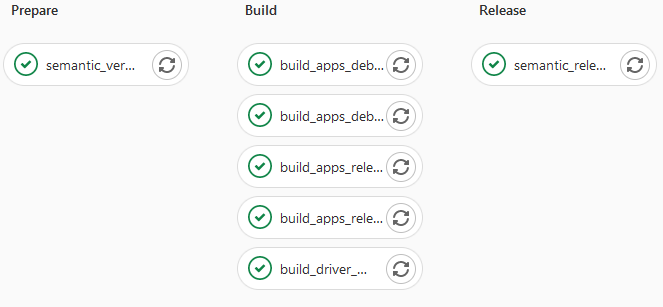
\includegraphics[width=\textwidth]{semantic_release_pipeline}
    \caption{Etapy procesu automatyzacji z~wykorzystaniem \emph{semantic-release}.}
    \label{fig:semantic_pipeline}
\end{figure}

Zasady dokonywanej przez \emph{semantic-release} analizy wiadomości, istniejącej w~ramach rewizji, zostały ustandaryzowane według konwencji \emph{ESLint} \cite{eslint}. W~przypadku, gdy powinno zostać utworzone nowe wydanie, należy wraz z~nową rewizją przygotować wiadomość w~następującym formacie: \lstinline{<tag>: <opis>}, gdzie \lstinline{<tag>} to jedna z~następujących wartości:
\begin{itemize}
    \item Fix - naprawa błędu
    \item Update - usprawnienie kompatybilne wstecz
    \item New - nowa funkcjonalność
    \item Breaking - zmiany niekompatybilne wstecz
    \item Docs - zmiany w~dokumentacji
    \item Build - zmiany w~procesie budowania
    \item Upgrade - zmiany w~zależnościach
    \item Chore - zmiany, które w~żaden sposób nie wpływają na użytkowanie, np.: zmiany w~testach
\end{itemize}
Opisem może być dowolna wiadomość krótko podsumowująca dokonane zmiany. Technologia \emph{semantic-release} ustala automatycznie na podstawie analizowanych tagów, stosując zasady \emph{semantic-versioning}, odpowiednią informację o~wersji. Przykładowe działania projektu \emph{semantic-release} zostało przedstawione na listingu \ref{lst:analyze}.

\lstinputlisting[
    language=Cmd, 
    caption={Analiza wiadomości zawartych w~rewizjach z~wykorzystaniem \emph{semantic-release}.}, 
    label={lst:analyze}
]{4_infrastructure/code_samples/analyze.txt}

\subsection{Podsumowanie}
Dzięki zastosowaniu wszystkich przedstawionych kroków stworzono w~projekcie GGSS scentralizowany, zautomatyzowany system wersjonowania wydań aplikacji. Wszystkie czynności potrzebne do utrzymania odpowiedniej wersji odbywają się w~ramach automatyzacji opartej o~GitLab CI/CD oraz projekt \emph{semantic-release}. Deweloper musi jedynie wprowadzać odpowiednie oznaczenia w~wiadomościach związanych z~kolejnymi rewizjami, a~utworzony system automatycznie zajmie się ewaluacją wszystkich trzech komponentów kolejnej wersji, zbuduje wszystkie komponenty systemu przekazując wcześniej uzyskane dane oraz udostępni gotowe do działania aplikacje w~ramach nowego wydania dostępnego na portalu GitLab.


\clearpage
\section{Pakietowanie i rozlokowanie projektu (JC)}
\label{ch:packages}

% Tutaj zmiany w skryptach opereracyjnych, trap na killera
% TODO: zmienić nazwę, np. Zmiany w infrastrukturze docelowej projektu


\subsection{Wprowadzenie do problematyki}

\subsection{Motywacja do wprowadzenia zmian}

\subsection{...}

\clearpage
\section{Rozwój infrastruktury do testowania warstwy sprzętowej (JC)}
\label{ch:hardware_testing}

Niniejsza część pracy została poświęcona aspektowi testowania urządzeń fizycznych wykorzystywanych przez projekt GGSS. Zostały omówione próby przygotowania infrastruktury pozwalającej na przeprowadzanie testów z~ominięciem głównej aplikacji GGSS oraz ostateczne rozwiązanie przyjęte przez autorów. Same testy aplikacji do testowania urządzeń zostały opisane w~ramach rozdziału \ref{cha:tests}.

\subsection{Wprowadzenie do problematyki}
Ze względu na to, że system GGSS do działania wymaga sprzętu fizycznego ważne jest, aby przed uruchomieniem głównej aplikacji była możliwość sprawdzenia, czy urządzenia są sprawne. System GGSS nie może zostać uruchomiony na niepoprawnie skonfigurowanym sprzęcie, ponieważ może to doprowadzić do różnych konsekwencji jak na przykład trwałe uszkodzenie urządzeń. Biorąc pod uwagę te wymogi w~ramach systemu GGSS istniały skrypty w~języku Python oraz aplikacja w~języku C++ służące do wykonywania akcji na sprzęcie fizycznym w~celu jego weryfikacji.

\subsection{Motywacja do wprowadzenia zmian}
Rozwiązanie dotychczas stosowane w~projekcie GGSS posiadało wiele mankamentów. Największą jego wadą była dodatkowa zależność do biblioteki \emph{python-serial}, która nie jest obecna w~środowisku docelowym przez co w~ramach instalacji pakietu projektu GGSS konieczna była instalacja również tejże biblioteki. Dodatkowo kod źródłowy był mało czytelny, przez co ciężko było rozszerzyć możliwości skryptów, szczególnie w~przypadku tych w~języku Python. Co więcej skrypty te wymagały rozszerzeń ze względu na swoje niewielkie możliwości weryfikacji sprzętu.

Autorzy postanowili rozwiązać te problemy tworząc nowe skrypty służące testowaniu urządzeń. Postawiono kilka celów, które te skrypty miały realizować. Po pierwsze najważniejszym założeniem było udostępnienie takiego interfejsu, który będzie pozwalał na możliwie jak najbardziej kompletne przetestowanie sprzętu znając jedynie komendy jakie ten sprzęt przyjmuje. Ważne, aby specjalista był w~stanie dogłębnie sprawdzić działanie sprzętu bez potrzeby zaglądania w~kod źródłowy skryptów służących do testowania. Kolejnym celem, który autorzy postanowili zrealizować, to zapewnić podobny interfejs w~przypadku wszystkich przygotowanych aplikacji. Ostatnim z~głównych celów było, w~miarę możliwości, pozbycie się jak największej ilości zewnętrznych zależności.

Po głębszej analizie potrzeb i~możliwości dotąd stosowanych aplikacji, autorzy zdecydowali się pozostawić aplikację do testowania \emph{analizatora wielokanałowego} w~stanie oryginalnym, a~skupić się na aplikacjach, których zadaniem jest testowanie \emph{zasilacza wysokiego napięcia} oraz \emph{multipleksera}. Opisowi zostały poddane jedyne te aplikacje oraz skrypty, które zostały stworzone, bądź zmodyfikowane przez autorów.

\subsection{Rozwiązanie oparte o~język Python}
W~celu ułatwienia pracy ze sprzętem postanowiono przygotować prosty skrypt współpracujący z~aplikacją \emph{udevadm} \cite{udevadm}, służącą do obsługi i~pobieraniu informacji z~systemu plików \emph{udev}, którego zadaniem jest dynamiczna alokacja plików urządzeń. Celem wyżej wymienionego skryptu było automatyczne pobieranie informacji na temat podłączonych do komputera urządzeń wchodzących w~skład projektu GGSS. Proces ten odbywał się za pomocą analizowania metadanych dostarczanych w~ramach działania aplikacji udevadm. Listing \ref{lst:device_detector} przedstawia przykładowe działanie skryptu służącego do wykrywania sprzętu. Najważniejszą informację jaką uzyskujemy w~ramach jego działania to ścieżki do plików urządzeń, które są parametrem wejściowym potrzebnym do działania, przygotowanych przez autorów, aplikacji do testowania sprzętu.

\lstinputlisting[
    language=Cmd, 
    caption={Przykład działania skryptu do automatycznego wykrywania podłączonych urządzeń}, 
    label={lst:device_detector}
]{4_infrastructure/code_samples/device_detector.txt}

Przygotowane zostały również dwie aplikacje w~języku Python. Jedna służąca do testowania multipleksera, a~druga do testowania zasilacza wysokiego napięcia. Docelowo obie aplikacje miały oferować tryb interaktywny, w~którym osoby pracujące nad systemem mogą wprowadzać wcześniej zdefiniowane komendy za pomocą wyżej wymienionych aplikacji, a~wynik ich działania byłby dostępny w~ramach informacji zwrotnej. Ze względu na ograniczenia czasowe w~ramach pierwszej implementacji jedynie aplikacja do testowania multipleksera oferowała taki tryb. Oprócz tego obie aplikacje oferowały zwykły tryb działania, tj.: wykonanie wcześniej zdefiniowanego zestawu komend oraz sprawdzenie poprawności ich wykonania i~informacji zwrotnych od sprzętu.

Rozwiązanie utworzone przez autorów realizowało tylko kilka celów, które zostały postawione. Po pierwsze częściowo został zrealizowany cel pozwalający na dogłębne przetestowanie sprzętu fizycznego. Ze względu na tryb interaktywny użytkownicy systemu byli w~stanie sprawdzić działanie w~różnych, wymyślonych przez siebie przypadkach. Dodatkowo nowo napisane aplikacje stosowały się do standardów co do tworzenia czystego, łatwo rozszerzalnego kodu stosowanych w~branży programistycznej, dzięki czemu dodawanie nowych funkcjonalności nie sprawiało dużych problemów.

Nie udało się natomiast pozbyć zależności do zewnętrznej zależności, jaką była biblioteka \emph{python-serial}. Co więcej interfejs obydwu aplikacji nie był jednolity, ze względu na brakujący tryb interaktywny aplikacji przeznaczonej do zasilacza wysokiego napięcia. W~trakcie prac nad aplikacjami odkryto również, że logika odpowiedzialna za obsługę komend zasilacza wysokiego napięcia istnieje już w~systemie w~postaci bibliotek w~języku C++. Ponowna implementacja w~języku Python powodowała duplikowanie odpowiedzialności oraz znaczne zwiększenie kosztów utrzymania.

Z~powodu wyżej wymienionych wad utworzonego rozwiązania postanowiono ponownie rozwiązać ten problem, tym razem z~wykorzystaniem języka C++ oraz zastosowaniem jeszcze lepiej zaplanowanego interfejsu służącego testowaniu.

\subsection{Rozwiązanie oparte o język C++}
Tworząc rozwiązanie oparte o~język C++ w~pierwszej kolejności wykonano odpowiedni plan interfejsu użytkownika tak, aby był on jak najbardziej przyjazny i~pozwalał na jak najlepsze przetestowanie sprzętu. Celem było stworzenie takiego interfejsu, aby od użytkownika wymagana była jedynie znajomość komend. W~tym celu postanowiono, na wzór rozwiązania w~języku Python, zaimplementować tryb interaktywny. Oprócz trybu interaktywnego zdecydowanie się również na tryb pozwalający na łatwą automatyzację procesu bez potrzeby każdorazowego wprowadzania komend do aplikacji. W~ramach wypracowanego rozwiązania postanowiono dodać do aplikacji tryb scenariuszowy. Pozwala on na wykonanie wcześniej zdefiniowanych komend w~ramach scenariuszów zdefiniowanych w~zewnętrznym pliku. W~celu osiągnięcia jak największej czytelności zdecydowano się zastosować format zbliżony do dobrze znanego formatu \emph{YAML} \cite{yaml}. Listing \ref{lst:examplary_scenario} przedstawia przykładowy plik z~dwoma scenariuszami. Każdy ze scenariuszy składa się z~kilku osobnych komend. Widoczne są również komentarze, których wsparcie dodano w~celu zmniejszenia progu wejściowego dla osób, które dopiero zaczynają korzystać z~tego rozwiązania.

\lstinputlisting[
    language=yaml, 
    caption={Przykładowy scenariusz w~formacie zbliżonym do \emph{YAML}}, 
    label={lst:examplary_scenario}
]{4_infrastructure/code_samples/examplary_scenario.txt}

Logika obsługi plików scenariuszowych została zawarta w~ramach biblioteki \emph{scenario-lib}. Korzystają z~niej dwie aplikacje to testowania sprzętu, tj.: \emph{high-voltage-service-app} oraz \emph{multiplexer-service-app}. Interfejs tych aplikacji jest możliwie zbliżony do siebie. Objawia się to między innymi w~argumentach wejściowych obydwu aplikacji. Następne parametry są dla nich wspólne:
\begin{itemize}
    \item \lstinline{--help} - wyświetla opis wszystkich parametrów wejściowych oraz aplikacji
    \item \lstinline{--dev-port} - ścieżka do pliku urządzeń, które odpowiada testowanemu sprzętowi
    \item \lstinline{--scenario-file} - ścieżka do pliku ze scenariuszami
    \item \lstinline{--scenarios} - nazwy scenariuszy z~wcześniej wskazanego pliku scenariuszowego, które mają zostać uruchomione
\end{itemize}

Parametry \lstinline{--scenario-file} oraz \lstinline{--scenarios} są opcjonalne. W~przypadku ich podania aplikacje są uruchamiane w~trybie scenariuszowym, w~przeciwnym wypadku w~trybie interaktywnym. Ze względu na specyfikę sprzętu aplikacja \emph{high-voltage-service-app} wymaga również podania, jako argument wejściowy, ilości modułów w~połączeniu łańcuchowym - argument \lstinline{--dev-modules}.

Komendy wspierane przez aplikację \emph{multiplexer-service-apps} są następujące:
\begin{itemize}
    \item \lstinline{getsn} - pobranie numeru seryjnego
    \item \lstinline{setch <numer kanału>}  - pozwala na ustawienie aktywnego kanału
    \item \lstinline{getch} - pobranie aktywnego kanału
    \item \lstinline{setgetch} - ustawienie aktywnego kanału, a~następnie pobranie w~celu weryfikacji
\end{itemize}

W~przypadku aplikacji \emph{high-voltage-service-app} wspierane są wszystkie komendy, które wspiera biblioteka \emph{hvcommand-lib}, a~zatem wszystkie komendy możliwe do wykonania na zasilaczu. Aplikacja pozwala ponadto na wykonanie ich w~różnych trybach:
\begin{itemize}
    \item zwykły - wykonanie komendy i~wyświetlenie odpowiedzi
    \item asercji - wykonanie komendy i~porównanie odpowiedzi do zadanej wartości. Komenda ta wspiera akcje jedynie na jednym elemencie zasilacza, czyli wynikiem działania musi być jedna wartość. W~celu skorzystania z~tego trybu należy poprzedzić komendę słowem kluczowym \lstinline{assert}, a~jako przyrostek wpisać oczekiwaną wartość
    \item asercji z~tolerancją - tryb ten działa dokładnie, jak wyżej opisany tryb asercji, natomiast poza oczekiwaną wartością należy podać również wartość parametru tolerancji.
\end{itemize}
Dodatkowo wspierana jest również komenda \lstinline{sleep}. W~przypadku obsługi zasilacza wysokiego napięcia wymagane jest odczekanie pewnego okresu czasu zanim ustawione wartości pojawią się na wyjściu zasilacza. Przykładowe działanie wyżej przedstawionych aplikacji zostanie przedstawione w~ramach przeprowadzonych testów, które zostały opisane w~ramach rozdziału \ref{cha:tests}.

\subsection{Podsumowanie}
Ostatecznie utworzone rozwiązanie testowania sprzętu fizycznego wykorzystywanego przez projekt GGSS spełniło wszystkie zakładane przez autorów cele. Z~powodzeniem wyeliminowano zależność do biblioteki zewnętrznej \emph{python-serial}. Napisane przez autorów aplikacje cechują się w~miarę uwspólnionym interfejsem, a~od użytkowników wymagana jest jedynie znajomość komend. Możliwe jest dogłębne przetestowanie urządzeń korzystając z~trybu interaktywnego, a~zautomatyzowanie tego procesu możliwe jest przy użyciu scenariuszy. Co więcej tryb scenariuszowy pozwala na zmianę działania automatycznego sprawdzania poprawności sprzętu bez potrzeby modyfikowania samych aplikacji, czy też ich ponownej kompilacji. Wystarczy jedynie napisać nowy scenariusz i~podać go jako parametr wejściowy.
